\chapter{Site specific, \PC based phylogenetic models outperform experimentally informed models and overcome their laboratory bias} 
\label{ch:phylogeny}

\clearpage
\pagebreak

This chapter is an early version of a paper to be submitted to Genome Biology and Evolution and co-authored with Michael A. Gilchrist and Brian C. O'Meara.\\
\newline
\newline
C. Landerer, B.C. O'Meara, M.A. Gilchrist, Phylogenetic model of stabilizing selection is more informative about site specific selection than extrapolation from laboratory estimates

\section{Abstract}
The ever increasing importance of phylogenetics has not been meet with the appropriate development in models.
Many commonly used phylogenetic models lack biological realism.
Models focused on nucleotides are agnostic to selection on higher level selection on codons or amino acids.
Amino acid models on the other hand lack the ability to properly account for mutations.
Codon models try to account for both, mutation and selection, but share that only a single substitution matrix is used, resulting in the same equilibrium frequency at each site.
Two novel models, \selac and \phydms, attempt to remedy this issue by either inferring site specific selection from the sequence data or use supplementary information on site specific selection.
Here we assess and compare the fit and adequacy of phylogenetic inferences made using supplementary information on selection with \selac, a novel codon model of stabilizing selection on amino acids.
We utilize site specific selection parameters for the $\beta$-lactamase TEM estimated via deep mutation scanning to supplement phylogenetic inference to 49 observed sequences.
Using AIC as a measure of model fit, we find that supplementary selection parameters improve model fit compared to classical models without site specific selection ($\DeltaAIC = 289$) but lack model adequacy.
We also highlight that this lack in model adequacy is likely due to biased laboratory conditions.
In contrast, \selac not only provides improved model fit over classical models without site specific selection ($\DeltaAIC = 871$) and experimentally supplemented models ($\DeltaAIC = 582$), it also shows improved model adequacy.
This indicates that the development of more realistic models is more promising than the usage of supplementary data for phylogenetic inference.

\newpage

Phylogenetic inference is of ever increasing importance across biology \citep{omeara2006,YangAndBourne2009,Ruprecht2017,SchwartzAndSchaffer2017}. 
Most common models used for phylogenetic inference are incorporated into powerful software packages such as RAxML \citep{raxml}, RevBayes \citep{revbayes}, or IQTree \citep{nguyen2015}
While commonly used models are fast and easy to use, they lack biological realism.

Phylogenetic models focused on the nucleotide composition such as GTR, or UNREST \citep{Tavare1986,Yang1994} are limited to mutation effects and are agnostic to any higher level selection on codons or amino acids.
Amino acid models like JTT \citep{jones1992}, BLOSSUM \citep{blossum}, or WAG \citep{whelan2001} attempt to describe the effects of natural selection, however, these do not properly account for mutations between nucleotides and are purely phenomenological.
In an attempt to remedy the shortcomings of nucleotide and amino acid models, codon models combine mutation between nucleotides and selection on the amino acids for which they code.
Most popular are the codon model by \citet{GoldmanAndYang1994} (\gy) and its derivatives.
However, \gy is commonly misinterpreted and provides only a restricted selection scenario that is best described as frequency dependent selection \citep{HughesAndNei1988,Nowak2006,Hughes2007,beaulieu2019}.

One common property of the aforementioned models is the fact that they use a single substitution model across all sites. As a result, every site, whether a nucleotide,  amino acid, or codon, have the same equilibrium distribution.
Biologists, however, have long recognized that equilibrium frequencies and thus the substitution matrix responsible, can vary substantially between sites \citep{felsenstein1981, gojobori1983}.
Individual sites along the sequence often show differences in evolutionary rates, and wide range of preferences for specific amino acids \citep{ashenberg2013, echave2016}.
In response, \citet{HalpernAndBruno1998} (\hb) provided a general, codon model were each codon site has its own, distinct substitution matrix.
The cost to this generality is the need for 19 amino acid specific selection parameters per site (N.B., the optimal amino acid, by definition, has a selection parameter of 0).
This need for estimating a large number of selection parameters from the sequence data makes the application of \citet{HalpernAndBruno1998} model unfeasible for most studies.
To overcome this parameterization problem,\citet{bloom2014} proposed using data from deep mutation scanning experiments (DMS) as a means of estimating the site specific parameters needed in the \citet{HalpernAndBruno1998}.
Bloom and others \citep{bloom2014, bloom2017, hilton2017} report that using DMS selection parameters greatly improves model fit over models without site specific selection parameters.

The power of DMS stems from the ability to manipulate a large number of individuals in the laboratory and estimate genotype fitness based on frequency changes over many generations.
This, however, limits the application of DMS selection parameters for phylogenetic inference to only organisms which can be cultured in the laboratory and with short generation times.
More troubling is the fact that variation between DMS experiments can lead to significant differences between model fits \citep{hilton2017}.
In addition, this inter-laboratory variation is likely small compared to the variation between laboratory conditions and those organisms usually encounter in the wild.
As a result, \emph{a priori} the value of DMS selection parameters for making inferences about sequences evolution in the wild is questionable.


An alternative to using laboratory based selection parameters to mitigate the parameterization issues introduced in \hb, an is to simplify the \hb model itself.
For example, Lartillot and colleagues mitigate the high numbers of  parameters required by \hb's codon model using a site categorization approach where a limited, but \emph{a priori} unspecified, number of site categories are estimated from the sequence data \citep{LartillotAndPhilippe2004,le2008,RodrigueEtAl2008,RodrigueAndLartillot2014}.
More recently, \citep{beaulieu2019} introduced a new codon model, \selac, where $20$ site categories are assumed \emph{a priori} to underlie the \hb model.
\selac combines \PC properties and site specific heterogeneity in the strength of selection together using a simplistic nested modeling approach.
Briefly, \selac infers an optimal amino acid for each site and then estimates the selection parameters for the remaining amino acids based on their \PC distance from the optimal amino acid and site specific sensitivity term which is, in turn, treated as a random effect.

We assess and compare the fit and adequacy of phylogenetic inferences made using supplementary DMS selection parameters and \selac. 
We use \phydms \citep{hilton2017} in order to utilize supplementary DMS selection parameters, fitting 49 TEM sequences observed in natural populations of \emph{E.~coli} presented in \citet{bloom2017}.
Following \citet{bloom2017, hilton2017}, we used the DMS based selection parameters from \citet{stiffler2016} for $\beta$-lactamase TEM to supplement our phylogenetic inference.
TEM is an enzyme found in gram-negative bacteria and catalyzes antibiotics with a $\beta$-lactam ring, providing antibiotic resistance \citep{Neu1969}.
The selection pressure imposed during the DMS experiment was limited to ampicillin and focused solely on the variant TEM-1 \citep{stiffler2016}.
However, TEM variants can also confer resistance to a wide range of other antibiotics \citep{sougakoff1988,sougakoff1989,goussard1991,mabilat1992,chanal1992,brun1994}.

Using AIC as a measure of model fit, as before we find that \phydms outperforms the 227 nucleotide and codon models included in the IQTree package \citep{bloom2014, bloom2017}, but that \selac outperforms \phydms by an additional 582 AIC units.
While very large, our estimate of \DeltaAIC between \selac and \phydms is likely an under estimate given the fact that we, conservatively, counted each inferred amino acid as a separate parameter when calculating \selac's AIC value.
In addition to a superior fit to the observed data, \selac shows higher model adequacy and implies more realistic values of genetic load than \phydms.
We attribute \phydms's poor model adequacy to laboratory bias in the DMS selection parameters.
This poor model adequacy, in turn, leads to the unrealistically large estimates of genetic load of the observed TEM sequences.

Together, our results indicate that models can be more informative and applicable than unnatural supplementary data for phylogenetic inference.
\selac, in contrast, provides biological meaningful information such as site specific optimal amino acids and estimates of selection parameters.
In addition, \selac does not rely on supplementary data, thus making it applicable to any protein coding sequence alignments, and can be expanded to test other hypothesis.

\section{Results}
\subsection{\selac Outperforms Experimentally Informed Models}

We compared \selac and \phydms, two models of site specific stabilizing selection, to 131 nucleotide and 97 codon uniform site models fitted using IQTree \citep[][see Table \ref{tab:AIC_selac} for the best performing models and Table \ref{tab:AIC_full} for all models]{nguyen2015}.
\selac shows the best model fit and provides an improvement of 582 AIC units over the empirically informed model fit by \phydms.
This better performance is in spite of the fact that \selac requires the specification of one optimal amino acid for each of the 263 codons in our TEM alignment.
The \phydms model, parameterized by site specific selection parameters from \citet{stiffler2016} performs second best and provides an improvement of 289 AIC units for the best uniform site model \emph{SYM+R2} (\emph{SYM}) \citet{zharkikh1994}. 
The best performing uniform codon model is the \emph{GY94+F1X4+R2} variant of \gy. 
In addition to \emph{SYM+R2}, \gy is outperformed by 109 other nucleotide models.
In contrast to \selac, which is a model of stabilizing selection, \gy is best interpreted as frequency dependent selection \citep{HughesAndNei1988,Nowak2006,Hughes2007,beaulieu2019}.

It is worth noting that of the $374$ parameters estimated by \selac, the vast majority, $263$, are discrete parameters corresponding to the optimal amino acid for each site.
These 263 discrete parameters are only $\sim5\%$ of the $19\times N = 4997$ parameters necessary to fully describe site specific selection.
Statistically speaking, it is unclear if \selac's discrete parameters contribute to the Kullback-Leibler divergence in a similar manner as continuous parameters.
As a result, it is possible that we are over penalizing \selac and thus our AIC and \DeltaAIC values underestimate \selac's performance.

\begin{table}
  \centering
  \caption{Comparison of the best performing models by category based on their AIC values, where  $\log(Lik)$ is the log-likelihood each model and $n$ is the number of model parameters estimated from the aligned sequence data.
    The two best performing models are the site specific models of amino acid stabilizing selection \selac and \phydms.
    The best performing nucleotide model is the variant of \citet{zharkikh1994}'s symmetrical model \emph{SYM+R2} with two rate categories. 
    The best performing codon model is the \emph{GY94+F1X4+R2} variant with unequal nucleotide frequencies but equal frequencies over all three codon positions and two rate categories.    
  See Table \ref{tab:AIC_full} for results from \selac, \phydms and all 227 other models tested.
}  
  \begin{tabular}{lrrrrrr}
    \hline
    Model							& $\log(Lik)$ & $n$ & AIC & \DeltaAIC \\ \hline 
    \selac							& -1498 & 374 & 3744 &  0 \\
    \phydms 						& -2061 & 102 & 4326 & 582 \\
    \emph{SYM+R2} 				& -2206 & 102 & 4615 & 871 \\
    \emph{GY94+F1X4+R2} 		& -2243 & 102 & 4690 & 946 \\ \hline
  \end{tabular}
  \label{tab:AIC_selac}
\end{table}


In addition to variation in model performance, we also observe differences in the topology between model fits.
Because the \selac model is too slow in its current form to feasibly identify the best tree topology, we fixed its topology to that estimated using the codon model of \citet{KosiolEtAl07}.
In order avoid biasing our results towards \selac, we used \selac's topology as an initial condition of our \phydms model fitting.
The fact that the best fitting \phydms parameterization diverges from the initial topology indicates our estimate of $\DeltaAIC$ between \selac and \phydms is conservative.
If we utilize the \phydms inferred topology with \selac, we find a very similar but slightly worse model fit to our original \selac fit ($\DeltaAIC = 2$).
This indicates that the topology has less impact on the model fit than the assumed optimal amino acid sequence, likely due to the short branches and many polytomies in the phylogeny (Figure \ref{fig:phylo_comp}).
Overall, Figure \ref{fig:phylo} shows that the estimated phylogenetic trees shift from long terminal branches (\selac) to longer internal branches (\phydms).
While the \selac model fit shows $84 \%$ of all evolution happening along the terminal branches, this reduces $77 \%$ in the \phydms and \gy model fits.
In addition, polytomies are widespread in all estimated phylogenies, and generally, the shortest branch length are estimated by \emph{SYM}.



\singlespacing
\begin{figure}[H]
     \centering
	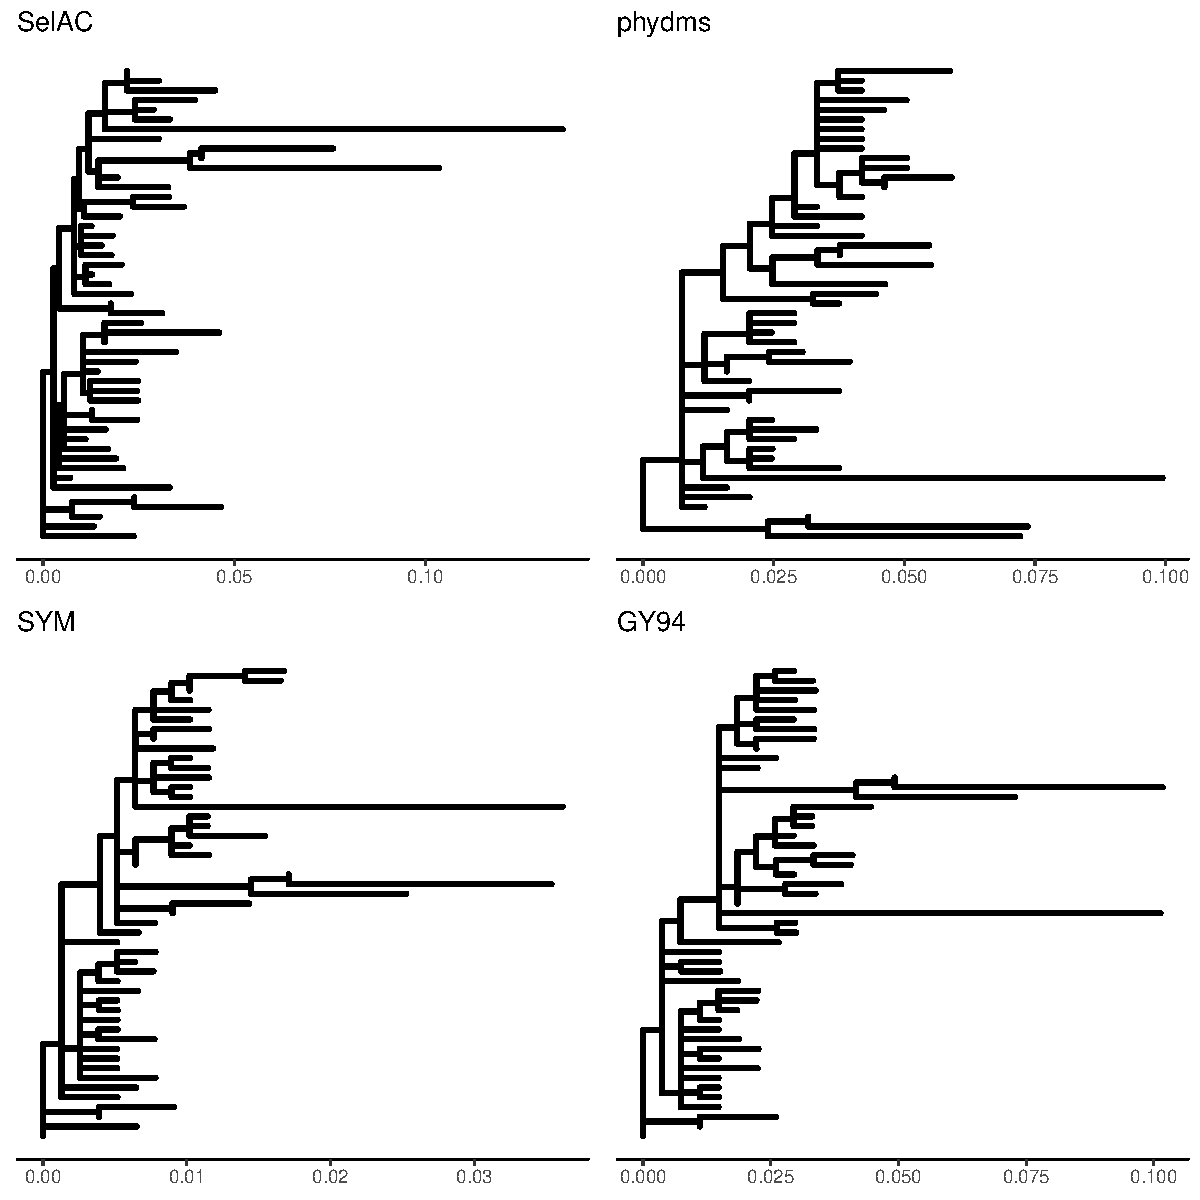
\includegraphics[width=\textwidth]{ch4/phy_TEM2016.pdf}
	\caption{Phylogenies resulting from \selac, phydms, \emph{SYM}+R2, and \emph{GY94}+F1X4+R2. As \selac is currently to slow for the inference of topologies, the topology for the \selac phylogeny was inferred using the codon model of \citet{KosiolEtAl07}.}
	\label{fig:phylo}
\end{figure}
\doublespacing
\clearpage

\subsection{\selac Improves Model Adequacy Over \phydms}

In order to evaluate the model adequacy of \selac and \phydms, we calculated the genetic loads of the observed TEM sequences under each model and compared them to their expected values generated by simulating the models.
More specifically, we simulated sequences forward in time from the ancestral state under the DMS and \selac inferred selection to establish a point of reference and further assess model adequacy.

\begin{figure}
    \centering
    \begin{subfigure}
        \centering
        (a)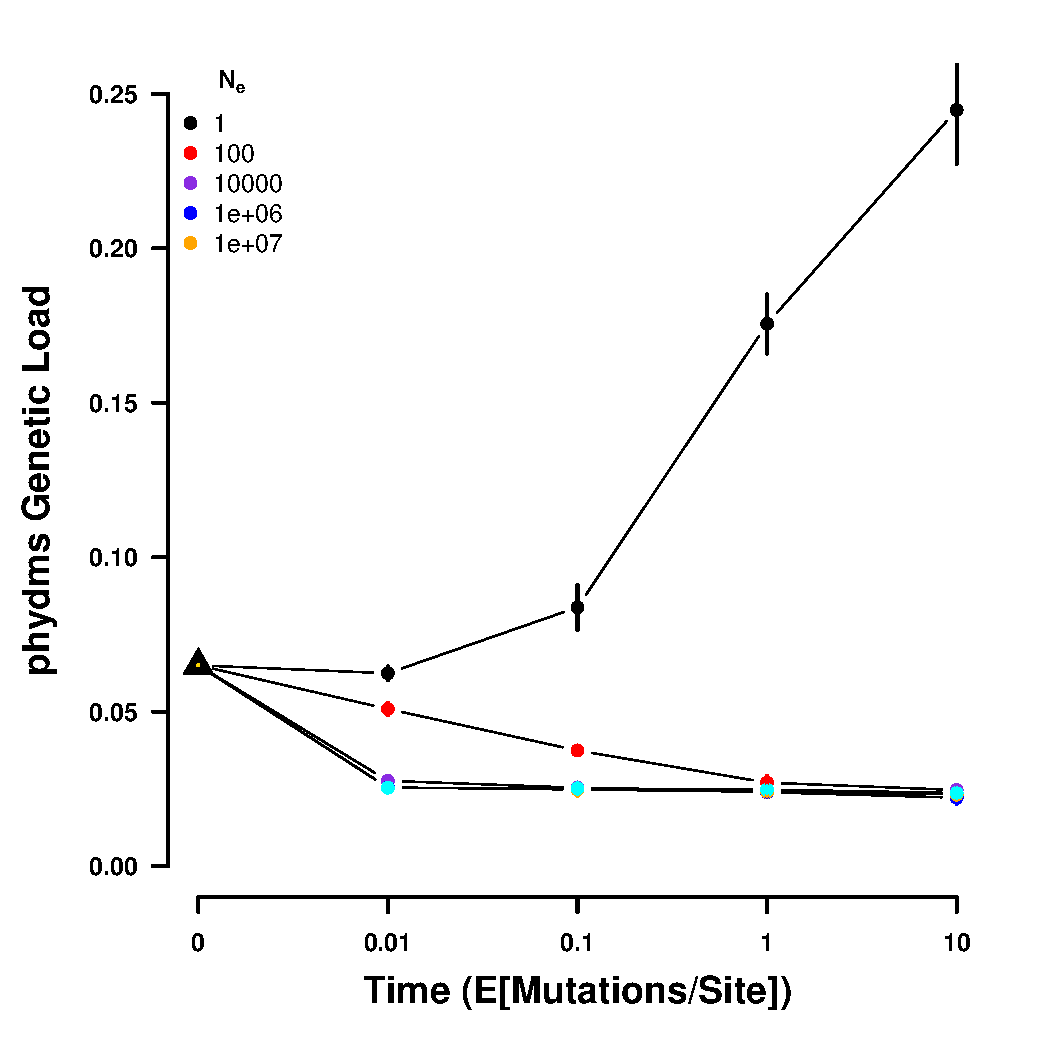
\includegraphics[width=.45\textwidth]{ch4/simulated_gl_time_DMS_ancest.pdf}
    \end{subfigure}
    \begin{subfigure}
        \centering
        (b)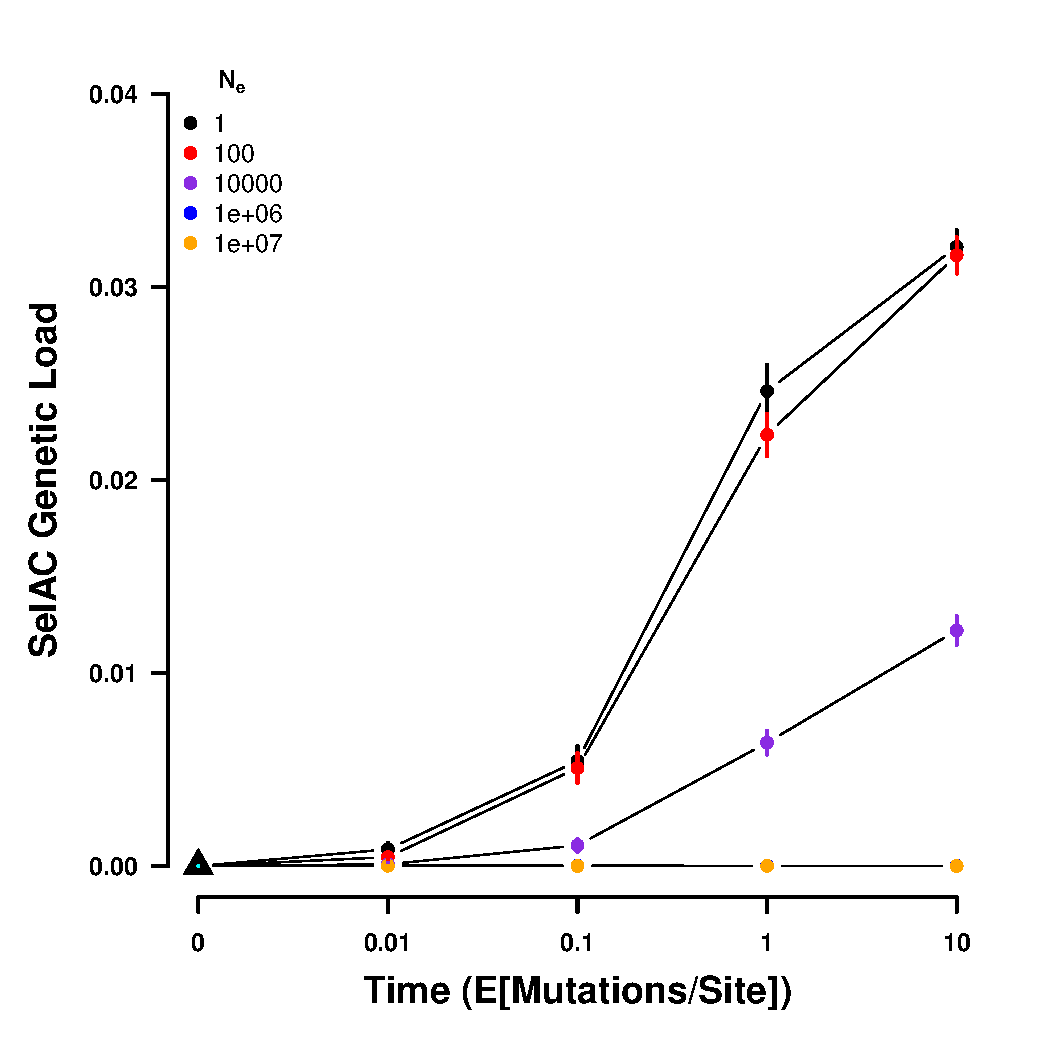
\includegraphics[width=.45\textwidth]{ch4/simulated_gl_time_SELAC_ancest.pdf}
    \end{subfigure}
    \caption{Sequences simulated from the ancestral state under the site specific selection on amino acids estimated using DMS (left) and \selac (right) at various times for a range of $N_e$ values.
    Time units are expected mutations per site, which equals the substitution rate of a neutral mutation.
    Points indicate sample means and vertical bars indicate standard deviations. Initial sequence is the inferred ancestral state of the TEM variants and indicated by a black triangle.}
    \label{fig:gl_sim}
\end{figure}

Simulations under the \phydms selection parameters show that the genetic load of the observed sequences is larger than the genetic load of the simulated sequences.
The simulation yields an average site specific genetic load of 0.025 (Figure \ref{fig:gl_sim}a).
Thus, even under the \phydms selection parameters, we would expect the observed sequences to show higher adaptation.
Simulations under the \selac inferred selection show that the genetic load of the observed sequences is less than the genetic load of the simulated sequences.
The simulation yields an average site specific genetic load of $1.3 \times 10^{-5}$ (Figure \ref{fig:gl_sim}b).
This appears to be near the selection-mutation-drift equilibrium and is consistent with theoretical population genetics (see Discussion).

Overall, the \selac fit shows high model adequacy and predicts a zero genetic load at invariant sites.
In contrast \phydms predicts a genetic load at these sites that is not significantly different from the genetic load at the variant sites (Table \ref{tab:selection}).
This shows that the distribution of genetic load differs between DMS inferred site specific selection and \selac inferred site specific selection.
If we assume the site specific selection parameters used in \phydms, 111 sites show no genetic load.
In contrast, if we assume the site specific selection estimated by \selac, 207 sites show no genetic load.
The \selac selection parameters are more in line with the observed sequences as only 66 sites show genetic variation.

The difference in the predictions of genetic load between \selac and DMS are caused by the difference of the \selac and DMS predicted sequences of selectively favored amino acids.
While the \selac sequence of selectively favored amino acids has $99 \%$ sequence similarity with the observed consensus sequence, the DMS predicted sequence only shows $52 \%$ similarity.
We also observe that 46 \% of the sites do not show the selectively favored amino acid at all.
For example, at site 157, we observe the non-polar, hydrophobic amino acids methionine, but the DMS experiment predicts that the polar, hydrophilic amino acid threonine provides the highest fitness.
Together our results suggests that the DMS selection parameters used in \phydms are not informative about selection in the wild and that \selac is a more appropriate tool to obtain such estimates.

\begin{table}
  \centering
  \caption{Genetic load at variant and invariant sites in the TEM alignment according to \selac and DMS}
  \begin{tabular}{lccc}
    \hline
			& 		& \multicolumn{2}{c}{Genetic Load}  \\ 
    Sites 		& \# Residues	& \multicolumn{1}{c}{\selac} & \multicolumn{1}{c}{DMS} \\ \hline 
    Variant	&	66	& $6.3\times10^{-7}$ & 0.010  \\
    Invariant		& 	197	& 0 & 0.007 \\
  \end{tabular}
  \label{tab:selection}
\end{table}





\section{Discussion}
We compared the performance of two codon level phylogenetic models with site specific selection, \phydms and \selac, as well as 227 more commonly used codon and nucleotide models in explaining 49 aligned TEM sequences obtained from \citet{bloom2017}.
Using AIC as measure of model fit we find that both models of site specific selection, \phydms and \selac perform substantially better that the alternative models (Table \ref{tab:AIC_selac}).
Further, we find that \selac substantially outperforms \phydms ($\DeltaAIC = 582$).

The improved performance of \phydms and \selac presumably results from their ability to more realistically describe the effects of natural selection on sequence evolution.
However, this realism comes at a cost. 
\phydms requires supplementary selection parameters for each amino acid at every site, which necessitates experimental work.
\selac, on the other hand, uses a nested modeling approach, which avoids the necessity of amino acid specific selection parameters, but greatly increases the computational cost of model fitting.

We further assess the model adequacy of \phydms and \selac which we primarily define as the similarity of the sequence of optimal amino acids to the observed consensus sequence.
While the consensus sequence ignores the phylogenetic relationship between the sequences, it is a still good metric to assess the realism of the estimated optimal amino acids as it provides a summary of the amino acids observed in the wild.
We also assess the genetic load of the observed sequences according to the DMS and \selac selection parameters.
Model adequacy is a measure that describes how well observed data can be reproduced by a model and is unfortunately often ignored.
Since the model adequacy of \phydms is a direct function of the supplementary DMS measurements we focus directly on these measurements.

Like model selection, model adequacy strongly favors \selac.
When we assess model adequacy by sequence similarity the sequence of optimal amino acids estimated by DMS has only 49 \% sequence similarity while the \selac estimated sequence shows a sequence similarity of 99 \% with the observed consensus sequence.
Given these results, it is tempting to assume that the consensus sequence will always fair best, however, this would assume independence between the observed sequences.
Furthermore, the high sequence similarity between the consensus sequence and the sequence of optimal amino acids is likely due to the high average sequence similarity in the TEM alignment of 98 \%.

Similarly, we find the genetic load of the DMS sequences is substantially higher when assuming the DMS estimated selection on amino acids compared to the \selac estimates with 0.065 and  $2.4\times 10^{-7}$, respectively.
However, if we assume that the DMS inference adequately reflects the evolution of TEM in the wild the observed sequences are either maladapted or were unable to reach a fitness peak.
This, however is unlikely as \ecoli has a large effective population size.
Estimates are on the order of $10^8$ to $10^9$ \citep{OchmanAndWilson1987,hartl1994}.
We would therefore expect that \ecoli can effectively explore the sequence space.
More specifically, assuming a mutation rate of $2.54\times 10^{-10}$ mutations per generation per nucleotide \citep{lee2012}, we would expect to find $2\times 10^{-7}$ mutations per generation in the 789 nucleotide long TEM sequence.
This results in between $\mu N_e = 10^1$ to $10^2$ mutations per generations throughout the population.
%The average site specific selection against the observed TEM sequences is $s = 0.085$, we would therefore expect that such a mutation should fix on average within $(4/|s|)\times \ln(2 N_e) \sim 1200$ to 1300 generations \citep{CrowAndKimura1970}.
%Given \ecoli's rapid doubling time of 15 hours in the wild \citep{gibson2018}, this means that such a mutation should spread through the population in 1.5 years.
However, this also clearly shows that the weak mutation assumptions made by all considered models, including \selac, is clearly violated.

In contrast, estimates of selection obtained by \selac show the observed sequences near a fitness peak.
%This is consistent with predictions discussed above.
It, therefore, appears that DMS reflects the biased laboratory selection on the TEM sequences with respect to only one antibiotic, ampicillin. 
This may be appropriate to model selection in a hospital environment, but not the evolution of TEM in the wild.
The evidence we derive from population genetics theory has us expecting the observed sequences at the selection-mutation-drift equilibrium.
This, however, is clearly not the case if we assume the DMS inferred selection.

Besides relatively poor performance in terms of model adequacy, DMS has additional shortcomings that limit its use in phylogenetic studies.
Like with any other experiment, results can greatly vary between laboratories.
\citet{hilton2017} showed that a similar experiment to the one used here by \citet{firnberg2014} performed worse in explaining the observed TEM data.
DMS experiments are also costly and limited to microorganisms that can be cultivated and manipulated under laboratory conditions.
These laboratory conditions can lead to the bias in selection parameters we show in this study.

The artificial selection environment in the laboratory leads to a very heterogeneous population and very large selection coefficients $s$ unlikely to be observed in the wild.
The very large single selection pressure may be the easiest issue to overcome in DMS experiments as it may be possible to include a multitude of weaker selective forces.
However, this is often not the goal when performing DMS experiments as they were designed to identify mutational effects in responds to specific selection.
\selac on the other hand, better explains the evolution of TEM in the wild and does not require selection parameters but instead provides such estimates from the sequence data.
This makes \selac also applicable to any set of aligned protein coding sequences.

However, \selac is  not without shortcomings itself, but its mechanistic nature provides direct avenues to overcome many of them via model expansion.
For example, \selac assumes invariance in the optimal amino acid at a site across the whole phylogeny.
This may be appropriate for closely related organisms in similar environments but not necessarily for distantly related species.
Incorporation of a hidden markov model would not only allow for shifts in the optimal amino acid along the phylogeny.
A hidden markov approach would also allow for frequency dependent selection like \gy.
Frequency dependent selection may be appropriate for certain TEM sites as it plays a role in chemical conflicts between microorganisms.
However, our results and the high number of invariant sites in the alignment indicate that such frequency dependent selection may only apply to a small number of sites.

In order to map the amino acid sequence to protein fitness \selac uses the euclidean distance in \PC space between amino acids. 
A more realistic mapping could be employed by adding higher order terms or by utilizing an explicit molecular model.
\selac also currently ignores selection on synonymous codon usage and therefore treats synonymous mutations as neutral.

Other shortcomings of \selac with a less clear solution include the relaxation of the constrained that the site specific sensitivity of selection has to be positive.
Allowing for a negative sensitivity term would extend \selac to diversifying selection on amino acids.
The inclusion of a mixture model where model parameters vary between site categories would allow to distinguish e.g. sites under stabilizing and diversifying selection.
Finally, \selac, like all other models considered here, assumes site independence, and thus ignores epistatic interaction between amino acids.

DMS experiments have been proposed to supplement information on selection on amino acids in phylogenetic studies.
Our study shows that this information on site specific selection parameters is unnecessary.
This is because the relevant information on stabilizing selection is already embedded within protein coding sequence alignments and can be inferred using a nested modeling approach.
In addition to being unnecessary, we show that DMS estimates of selection parameters are unnaturally biased towards laboratory conditions.
The ability to expand \selac as outlined above make it a valid starting point for such improvements and allow for explicit hypothesis testing.
Taken together, our results indicate that efforts in improving phylogenetic inferences are likely better spent on the development of more realistic models rather than generating and/or incorporating DMS data.


\section{Materials and Methods}

\subsection{Phylogenetic Inference and Model selection}

Aligned TEM sequences were obtained from \citet{bloom2017}
Experimentally selection parameters for TEM were taken from \citet{stiffler2016}.
We followed \citep{bloom2017} and used the experimental selection parameters to determine site specific equilibrium frequencies for \phydms. 
\phydms (version 2.5.1) was fitted to the site specific selection from \citet{stiffler2016} using python (version 3.6).
\selac (version 1.6.1) was fitted to the TEM alignment using R (version 3.4.1) \citep{rcore}.
We assumed the \PC properties estimated by \citet{grantham1974} and only estimated the weighting terms for each property from the data.
We choose the constraint free, general unrestricted model (UNREST) \citep{Yang1994} as mutation model for \selac.
All other models were fitted using IQTree \citep{nguyen2015}.
All models were fitted using maximum likelihood.
We report each model's log likelohood ($\log(Lik)$), and AIC.


\subsection{Sequence Simulation}

Sequences were simulated by stochastic simulations using a Gillespie algorithm \citep{gillespie1976}.
Fixation probabilities were based on \citet{SellaAndHirsh2005}.
The selection parameters were estimated using \selac or taken from \citet{stiffler2016}.
We choose the selection parameters resulting from the highest concentration (2500 $\mu g/mL$) treatment of ampicillin for our comparison.
We rescaled the experimental selection parameters such that the amino acid with the highest fitness at each site has a value of one.
Mutation rates for the simulations were taken from the \selac.
The initial sequences was the ancestral sequence reconstructed using FastML \citep{fastml} (last accessed: 30.09.2018).
Each sequence was simulated 10 times and we report average genetic load and sequence similarity and the standard error.
The sequences were sampled at times 0.01, 0.1, 1, and 10 expected mutations per site.

\subsection{Estimating site specific selection parameters $w_i$}

Following \citet{beaulieu2019} $w_i$ is proportional to
\begin{equation}
w_i \propto \exp(-A_0\eta\psi)
\end{equation}
where $A_0$ describes the decline in fitness with each high energy phosphate bond wasted per unit time, and $\psi$ is the protein's production rate.
$\eta$ is the cost/benefit ratio of a protein (see \citep{beaulieu2019} for details). 
However, \selac only estimates a composition parameter $\psi' = A_0\psi N_e$ thus
\begin{equation}
\psi = \frac{\psi'}{A_0N_eq}
\end{equation}
\selac assumes that the effective population size $N_e = 5\times 10^6$ and that $A_0 = 4 \times 10^{-7}$ \citep{gilchrist2007}.

\subsection{Model Adequacy}

Model adequacy was assessed by comparing the observed sequences and simulations under the site specific selection inferred by the deep mutation scanning experiment or \selac.
First, similarity between the sequence of selectively favored amino acids and the observed TEM sequences was assessed.
Sequence similarity was measured as the number of differences in the aligned amino acid sequences.
Second, the genetic load of the observed and the simulated sequences was calculated using either the site specific selection inferred by the deep mutation scanning experiment or \selac.
The average genetic load for site $i$ in the alignment was calculated as
\begin{equation}
L_i = \frac{w_{max,i} - \overline{w_i}}{w_{max,i}}
\end{equation}
where $w_{max,i}$ is the fitness of the selectively favored amino acids at position $i$, either estimated using the site specific selection inferred by DMS or \selac.
$\overline{w_i}$ represents the average fitness of the residues observed at position $i$.
The average sequence specific genetic load $L$ was calculated as the sum of the site specific genetic loads $L = \frac{1}{n}\sum_{i=1}^n L_i$ where $n$ is the number of amino acid sites.

\section{Acknowledgments}
This work was supported in part by NSF Award and DEB-1355033 (BCO, MAG, and Russell Zaretzki) with additional support from the University of Tennessee Knoxville. 
CL received additional support as a Graduate Student Fellow at the National Institute for Mathematical and Biological Synthesis, an Institute sponsored by the National Science Foundation through NSF Award DBI-1300426, with additional support from UTK. 
The authors would like to thank Russell Zaretzki, Jeremy Beaulieu, and Alexander Cope for their helpful criticisms and suggestions for this work.


\clearpage

\section{Appendix: Supplementary Material}

The \selac inferred sequence of selectively favored amino acids has $99 \%$ sequence similarity with the observed consensus sequence.
This may not be to surprising given that \selac only uses the sequence data and no experimental supplementary data.
Simulations support the better model adequacy of \selac, however the decline in sequences sequence similarity to $83 \%$, indicating that \selac underestimates the strength of selection (Figure \ref{fig:dis_sim}b).

The sequence of selectively favored amino acids experimentally estimated by DMS shows a low sequence similarity of only $52 \%$ with the observed consensus sequence. 
We find that the selectively favored amino acid estimated by DMS is not found in the wild in 46.4 \% of sites.
Additionally, the \PC properties appear to differ between the observed and the DMS estimated optimal amino acids.
Simulations of codon sequences under the DMS inferred site specific selection further highlights that we would not expect to see the observed TEM sequences under these conditions.
We find that the simulated sequences show up to $62 \%$ sequence similarity to the observed consensus sequence (Figure \ref{fig:dis_sim}a).
This is a 10 \% higher sequence similarity than the sequence of selectively favored amino acids estimated by DMS have with the observed consensus sequence. 

A more detailed analysis shows that we find 100 sites where \selac predicts a genetic load of zero but the DMS estimates predict a non-zero genetic load.
All 100 cases show a significant difference in the likelihood between the \selac and the DMS inferred optimal amino acid given the observed sequence data.
In addition, these 100 sites show a significant higher average genetic load than the remaining 163 sites of $0.0157$ and $0.003$, respectively (paired t-test, $p = 3\times10^{-13}$).
For 52 sites, both \phydms and \selac estimate a non-zero genetic load.
In half the cases, the same optimal amino acid is predicted, in the remaining half \phydms predicts a significantly different optimal amino acid.
Again we find a significant difference in genetic load between the half for which the \selac and \phydms predictions of the optimal amino acid agree and the half for which they differ of $0.004$ and $0.0158$, respectively (paired t-test, $p = 2\times 10^{-5}$).
The site specific selection estimated by DMS for the observed TEM sequences represents an average site specific load of 0.065.
In contrast, the site specific genetic load estimated by \selac for the observed TEM sequences represents an average site specific genetic load of only $2.4\times 10^{-7}$.


\begin{figure}
    \centering
    \begin{subfigure}
        \centering
       (a)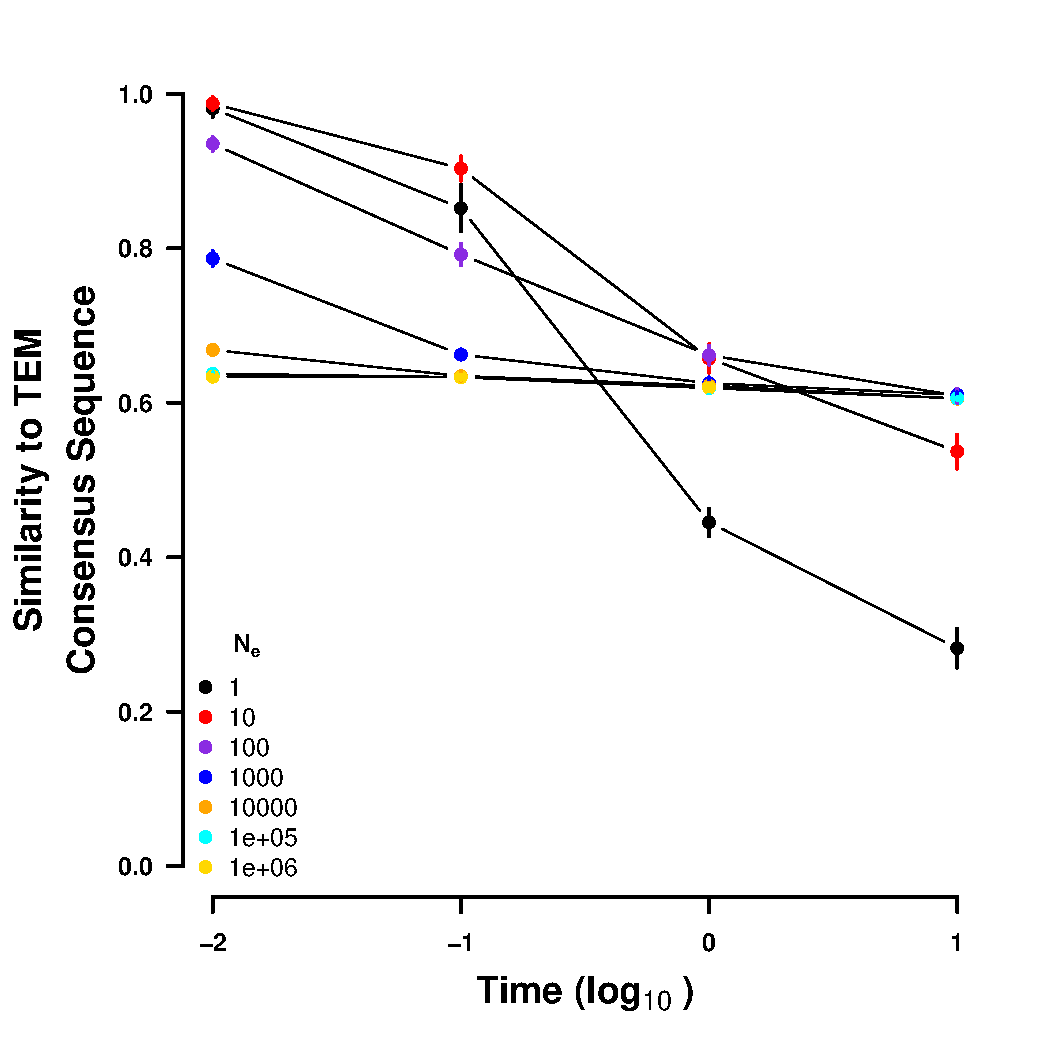
\includegraphics[width=.45\textwidth]{ch4/simulated_dist_time_DMS_ancest.pdf}
    \end{subfigure}
    \begin{subfigure}
        \centering
        (b)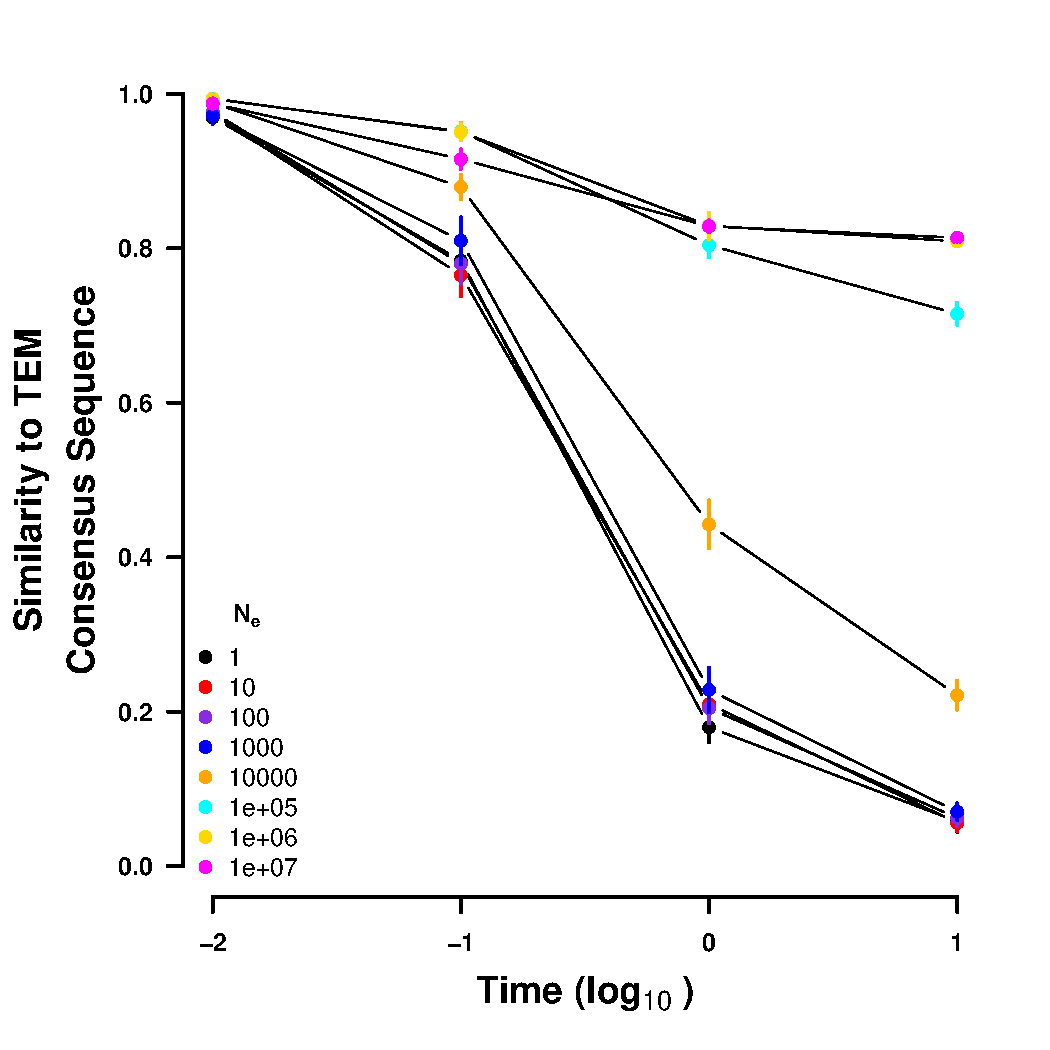
\includegraphics[width=.45\textwidth]{ch4/simulated_dist_time_SELAC_ancest.pdf}
    \end{subfigure}
    \caption{Sequences simulated from the ancestral state under the site specific selection on amino acids estimated using DMS (left) and \selac (right) at various times for a range of $N_e$ values.
    Time units are expected mutations per site, which equals the substitution rate of a neutral mutation.
    Points indicate sample means and vertical bars indicate standard deviations. Initial sequence is the inferred ancestral state of the TEM variants and indicated by a black triangle.}
    \label{fig:dis_sim}
\end{figure}

\clearpage

\singlespacing
\begin{longtable}{clrrrrrr}
  \caption{Model selection of 229 models of nucleotide and codon evolution.}
  \label{tab:AIC_full}
  \\ 
  \toprule
  No. & Model & $\log(Lik)$ & n & AIC & \DeltaAIC  \\   \hline \endfirsthead
  \caption*{Table \ref{tab:AIC_full} Continued}\\\toprule
  No. & Model & $\log(Lik)$ & n & AIC & \DeltaAIC  \\   \hline \endhead
  \hline \endfoot
  \bottomrule
  \endlastfoot

	1 & \selac+G4 & -1497.971 & 374 & 3743.942 & 0 \\ 
	2 & \phydms & -2060.85 & 102 & 4325.7 & 582 \\ 
	3 & SYM+R2 & -2205.877 & 102 & 4615.754 & 871.754 \\ 
	4 & TIMe+R2 & -2232.406 & 100 & 4664.811 & 920.811 \\ 
	5 & TVMe+R2 & -2232.838 & 101 & 4667.677 & 923.677 \\ 
	6 & TIM3e+R2 & -2234.332 & 100 & 4668.664 & 924.664 \\ 
	7 & TIM2e+R2 & -2234.381 & 100 & 4668.763 & 924.763 \\ 
	8 & K3P+R2 & -2235.777 & 99 & 4669.553 & 925.553 \\ 
	9 & TNe+R2 & -2236.078 & 99 & 4670.155 & 926.155 \\ 
	10 & SYM+R3 & -2229.616 & 104 & 4667.232 & 923.232 \\ 
	11 & TIM+F+R2 & -2230.958 & 103 & 4667.915 & 923.915 \\ 
	12 & TIMe+R3 & -2232.404 & 102 & 4668.808 & 924.808 \\ 
	13 & GTR+F+R2 & -2228.537 & 105 & 4667.073 & 923.073 \\ 
	14 & K3Pu+F+R2 & -2232.617 & 102 & 4669.234 & 925.234 \\ 
	15 & TVM+F+R2 & -2230.105 & 104 & 4668.21 & 924.21 \\ 
	16 & TVMe+R3 & -2232.838 & 103 & 4671.676 & 927.676 \\ 
	17 & K2P+R2 & -2239.424 & 98 & 4674.847 & 930.847 \\ 
	18 & TIM3e+R3 & -2234.332 & 102 & 4672.664 & 928.664 \\ 
	19 & TIM2e+R3 & -2234.381 & 102 & 4672.762 & 928.762 \\ 
	20 & TIM3+F+R2 & -2233.064 & 103 & 4672.127 & 928.127 \\ 
	21 & TIM2+F+R2 & -2233.114 & 103 & 4672.227 & 928.227 \\ 
	22 & K3P+R3 & -2235.777 & 101 & 4673.553 & 929.553 \\ 
	23 & TN+F+R2 & -2234.624 & 102 & 4673.249 & 929.249 \\ 
	24 & TPM3u+F+R2 & -2234.673 & 102 & 4673.347 & 929.347 \\ 
	25 & TPM3+F+R2 & -2234.674 & 102 & 4673.348 & 929.348 \\ 
	26 & TPM2u+F+R2 & -2234.681 & 102 & 4673.363 & 929.363 \\ 
	27 & TPM2+F+R2 & -2234.683 & 102 & 4673.365 & 929.365 \\ 
	28 & TNe+R3 & -2236.077 & 101 & 4674.155 & 930.155 \\ 
	29 & TIM+F+R3 & -2230.958 & 105 & 4671.915 & 927.915 \\ 
	30 & HKY+F+R2 & -2236.266 & 101 & 4674.531 & 930.531 \\ 
	31 & GTR+F+R3 & -2228.536 & 107 & 4671.073 & 927.073 \\ 
	32 & K3Pu+F+R3 & -2232.617 & 104 & 4673.234 & 929.234 \\ 
	33 & TVM+F+R3 & -2230.105 & 106 & 4672.21 & 928.21 \\ 
	34 & K2P+R3 & -2239.192 & 100 & 4678.384 & 934.384 \\ 
	35 & TIM3+F+R3 & -2233.063 & 105 & 4676.127 & 932.127 \\ 
	36 & TIM2+F+R3 & -2233.113 & 105 & 4676.227 & 932.227 \\ 
	37 & TN+F+R3 & -2234.624 & 104 & 4677.249 & 933.249 \\ 
	38 & TPM3u+F+R3 & -2234.673 & 104 & 4677.347 & 933.347 \\ 
	39 & TPM3+F+R3 & -2234.674 & 104 & 4677.348 & 933.348 \\ 
	40 & TPM2u+F+R3 & -2234.681 & 104 & 4677.363 & 933.363 \\ 
	41 & TPM2+F+R3 & -2234.682 & 104 & 4677.364 & 933.364 \\ 
	42 & HKY+F+R3 & -2236.074 & 103 & 4678.148 & 934.148 \\ 
	43 & SYM+I+G4 & -2243.212 & 102 & 4690.424 & 946.424 \\ 
	44 & TVMe+I+G4 & -2244.533 & 101 & 4691.066 & 947.066 \\ 
	45 & TIMe+I+G4 & -2246.457 & 100 & 4692.914 & 948.914 \\ 
	46 & K3P+I+G4 & -2248.166 & 99 & 4694.332 & 950.332 \\ 
	47 & TVM+F+I+G4 & -2241.853 & 104 & 4691.707 & 947.707 \\ 
	48 & TIM3e+I+G4 & -2247.379 & 100 & 4694.758 & 950.758 \\ 
	49 & K3Pu+F+I+G4 & -2245.156 & 102 & 4694.311 & 950.311 \\ 
	50 & GTR+F+I+G4 & -2241.484 & 105 & 4692.968 & 948.968 \\ 
	51 & TIM+F+I+G4 & -2244.418 & 103 & 4694.836 & 950.836 \\ 
	52 & TPM3u+F+I+G4 & -2246.03 & 102 & 4696.06 & 952.06 \\ 
	53 & TPM3+F+I+G4 & -2246.069 & 102 & 4696.138 & 952.138 \\ 
	54 & TIM2e+I+G4 & -2248.934 & 100 & 4697.868 & 953.868 \\ 
	55 & TNe+I+G4 & -2250.587 & 99 & 4699.174 & 955.174 \\ 
	56 & TIM3+F+I+G4 & -2245.534 & 103 & 4697.068 & 953.068 \\ 
	57 & K2P+I+G4 & -2252.181 & 98 & 4700.362 & 956.362 \\ 
	58 & TPM2u+F+I+G4 & -2247.579 & 102 & 4699.158 & 955.158 \\ 
	59 & TPM2+F+I+G4 & -2247.685 & 102 & 4699.371 & 955.371 \\ 
	60 & HKY+F+I+G4 & -2249.065 & 101 & 4700.13 & 956.13 \\ 
	61 & TIM2+F+I+G4 & -2247.009 & 103 & 4700.018 & 956.018 \\ 
	62 & TN+F+I+G4 & -2248.511 & 102 & 4701.023 & 957.023 \\ 
	63 & TVMe+I & -2254.804 & 100 & 4709.608 & 965.608 \\ 
	64 & K3P+I & -2257.72 & 98 & 4711.439 & 967.439 \\ 
	65 & SYM+I & -2254.11 & 101 & 4710.221 & 966.220 \\ 
	66 & TIMe+I & -2257.074 & 99 & 4712.149 & 968.149 \\ 
	67 & TVM+F+I & -2252.157 & 103 & 4710.315 & 966.315 \\ 
	68 & K3Pu+F+I & -2254.856 & 101 & 4711.712 & 967.712 \\ 
	69 & TIM3e+I & -2257.796 & 99 & 4713.592 & 969.592 \\ 
	70 & TPM3+F+I & -2255.771 & 101 & 4713.543 & 969.543 \\ 
	71 & TPM3u+F+I & -2255.771 & 101 & 4713.543 & 969.543 \\ 
	72 & K2P+I & -2261.218 & 97 & 4716.436 & 972.436 \\ 
	73 & GTR+F+I & -2252.067 & 104 & 4712.133 & 968.133 \\ 
	74 & TIM+F+I & -2254.783 & 102 & 4713.566 & 969.566 \\ 
	75 & TNe+I & -2260.579 & 98 & 4717.158 & 973.158 \\ 
	76 & TIM3+F+I & -2255.684 & 102 & 4715.368 & 971.368 \\ 
	77 & HKY+F+I & -2258.352 & 100 & 4716.703 & 972.703 \\ 
	78 & TIM2e+I & -2259.878 & 99 & 4717.757 & 973.757 \\ 
	79 & TVMe+G4 & -2258.853 & 100 & 4717.705 & 973.705 \\ 
	80 & SYM+G4 & -2257.573 & 101 & 4717.146 & 973.146 \\ 
	81 & TPM2+F+I & -2257.712 & 101 & 4717.423 & 973.423 \\ 
	82 & TPM2u+F+I & -2257.712 & 101 & 4717.423 & 973.423 \\ 
	83 & K3P+G4 & -2261.922 & 98 & 4719.844 & 975.844 \\ 
	84 & TIMe+G4 & -2260.683 & 99 & 4719.365 & 975.365 \\ 
	85 & TN+F+I & -2258.28 & 101 & 4718.561 & 974.561 \\ 
	86 & TIM3e+G4 & -2261.255 & 99 & 4720.51 & 976.51 \\ 
	87 & TVM+F+G4 & -2256.108 & 103 & 4718.216 & 974.216 \\ 
	88 & TIM2+F+I & -2257.643 & 102 & 4719.286 & 975.286 \\ 
	89 & K3Pu+F+G4 & -2258.971 & 101 & 4719.941 & 975.941 \\ 
	90 & TPM3u+F+G4 & -2259.716 & 101 & 4721.433 & 977.433 \\ 
	91 & TPM3+F+G4 & -2259.717 & 101 & 4721.434 & 977.434 \\ 
	92 & GTR+F+G4 & -2255.75 & 104 & 4719.5 & 975.5 \\ 
	93 & TIM+F+G4 & -2258.638 & 102 & 4721.276 & 977.276 \\ 
	94 & K2P+G4 & -2265.454 & 97 & 4724.907 & 980.907 \\ 
	95 & TNe+G4 & -2264.219 & 98 & 4724.437 & 980.437 \\ 
	96 & TIM3+F+G4 & -2259.366 & 102 & 4722.732 & 978.732 \\ 
	97 & TIM2e+G4 & -2263.57 & 99 & 4725.141 & 981.141 \\ 
	98 & JC+R2 & -2266.233 & 97 & 4726.466 & 982.466 \\ 
	99 & F81+F+R2 & -2262.327 & 100 & 4724.654 & 980.654 \\ 
	100 & HKY+F+G4 & -2262.499 & 100 & 4724.999 & 980.999 \\ 
	101 & TPM2+F+G4 & -2261.915 & 101 & 4725.829 & 981.829 \\ 
	102 & TPM2u+F+G4 & -2261.915 & 101 & 4725.829 & 981.829 \\ 
	103 & TN+F+G4 & -2262.169 & 101 & 4726.338 & 982.338 \\ 
	104 & TIM2+F+G4 & -2261.585 & 102 & 4727.17 & 983.17 \\ 
	105 & F81+F+R3 & -2262.028 & 102 & 4728.056 & 984.056 \\ 
	106 & JC+R3 & -2265.997 & 99 & 4729.994 & 985.994 \\ 
	107 & F81+F+I+G4 & -2274.845 & 100 & 4749.69 & 1005.69 \\ 
	108 & JC+I+G4 & -2279.318 & 97 & 4752.636 & 1008.636 \\ 
	109 & F81+F+I & -2283.56 & 99 & 4765.119 & 1021.119 \\ 
	110 & JC+I & -2287.984 & 96 & 4767.968 & 1023.968 \\ 
	111 & F81+F+G4 & -2287.834 & 99 & 4773.669 & 1029.669 \\ 
	112 & JC+G4 & -2292.095 & 96 & 4776.19 & 1032.19 \\ 
	113 & \gy+F1X4+R2 & -2242.963 & 102 & 4689.926 & 945.926 \\ 
	114 & MGK+F1X4+R2 & -2243.111 & 102 & 4690.221 & 946.221 \\ 
	115 & \gy+F1X4+R3 & -2238.022 & 104 & 4684.043 & 940.043 \\ 
	116 & MGK+F3X4+R2 & -2229.923 & 108 & 4675.846 & 931.846 \\ 
	117 & \gy+F1X4+I+G4 & -2247.179 & 102 & 4698.359 & 954.359 \\ 
	118 & MGK+F1X4+I+G4 & -2247.292 & 102 & 4698.583 & 954.583 \\ 
	119 & MGK+F1X4+R3 & -2241.989 & 104 & 4691.978 & 947.978 \\ 
	120 & MGK+F3X4+R3 & -2224.78 & 110 & 4669.559 & 925.559 \\ 
	121 & \gy+F1X4+G4 & -2251.144 & 101 & 4704.287 & 960.287 \\ 
	122 & MGK+F1X4+G4 & -2251.472 & 101 & 4704.944 & 960.944 \\ 
	123 & \gy+F3X4+R3 & -2227.048 & 110 & 4674.096 & 930.096 \\ 
	124 & \gy+F3X4+R2 & -2233.068 & 108 & 4682.136 & 938.136 \\ 
	125 & MGK+F3X4+I+G4 & -2233.539 & 108 & 4683.078 & 939.0781 \\ 
	126 & MGK+F3X4+G4 & -2237.512 & 107 & 4689.024 & 945.024 \\ 
	127 & \gy+F3X4+I+G4 & -2238.243 & 108 & 4692.485 & 948.485 \\ 
	128 & \gy+F3X4+R4 & -2227.106 & 112 & 4678.213 & 934.213 \\ 
	129 & \gy+F3X4+G4 & -2242.394 & 107 & 4698.789 & 954.789 \\ 
	130 & \gy+F1X4+I & -2260.085 & 101 & 4722.169 & 978.169 \\ 
	131 & MGK+F1X4+I & -2260.345 & 101 & 4722.69 & 978.69 \\ 
	132 & MGK+F3X4+I & -2246.112 & 107 & 4706.225 & 962.225 \\ 
	133 & MG+F1X4+R2 & -2268.482 & 101 & 4738.963 & 994.963 \\ 
	134 & \gy+F3X4+I & -2252.532 & 107 & 4719.064 & 975.064 \\ 
	135 & MG+F3X4+R2 & -2254.453 & 107 & 4722.906 & 978.906 \\ 
	136 & MG+F1X4+I+G4 & -2272.057 & 101 & 4746.113 & 1002.113 \\ 
	137 & MG+F1X4+R3 & -2267.523 & 103 & 4741.047 & 997.047 \\ 
	138 & MG+F1X4+G4 & -2276.171 & 100 & 4752.342 & 1008.342 \\ 
	139 & MG+F3X4+I+G4 & -2257.945 & 107 & 4729.891 & 985.891 \\ 
	140 & MG+F3X4+G4 & -2261.949 & 106 & 4735.898 & 991.898 \\ 
	141 & MG+F3X4+R3 & -2253.514 & 109 & 4725.027 & 981.027 \\ 
	142 & SYM & -2329.878 & 100 & 4859.756 & 1115.756 \\ 
	143 & TIMe & -2333.105 & 98 & 4862.21 & 1118.21 \\ 
	144 & TIM3e & -2333.481 & 98 & 4862.961 & 1118.961 \\ 
	145 & TVMe & -2333.164 & 99 & 4864.328 & 1120.328 \\ 
	146 & GTR+F & -2328.404 & 103 & 4862.809 & 1118.809 \\ 
	147 & K3P & -2336.391 & 97 & 4866.783 & 1122.783 \\ 
	148 & MG+F1X4+I & -2284.946 & 100 & 4769.892 & 1025.892 \\ 
	149 & TVM+F & -2330.086 & 102 & 4864.172 & 1120.172 \\ 
	150 & TIM+F & -2331.48 & 101 & 4864.96 & 1120.96 \\ 
	151 & TNe & -2336.729 & 97 & 4867.458 & 1123.458 \\ 
	152 & K3Pu+F & -2333.162 & 100 & 4866.323 & 1122.323 \\ 
	153 & TIM3+F & -2331.971 & 101 & 4865.942 & 1121.942 \\ 
	154 & TPM3+F & -2333.648 & 100 & 4867.297 & 1123.297 \\ 
	155 & TPM3u+F & -2333.648 & 100 & 4867.297 & 1123.297 \\ 
	156 & TIM2e & -2336.292 & 98 & 4868.584 & 1124.584 \\ 
	157 & MG+F3X4+I & -2270.442 & 106 & 4752.885 & 1008.885 \\ 
	158 & K2P & -2340.015 & 96 & 4872.03 & 1128.03 \\ 
	159 & TN+F & -2335.102 & 100 & 4870.204 & 1126.204 \\ 
	160 & HKY+F & -2336.783 & 99 & 4871.566 & 1127.566 \\ 
	161 & TIM2+F & -2334.7 & 101 & 4871.401 & 1127.401 \\ 
	162 & TPM2u+F & -2336.381 & 100 & 4872.761 & 1128.761 \\ 
	163 & TPM2+F & -2336.381 & 100 & 4872.762 & 1128.762 \\ 
	164 & JC & -2366.286 & 95 & 4922.571 & 1178.571 \\ 
	165 & F81+F & -2362.554 & 98 & 4921.108 & 1177.108 \\ 
	166 & \gy+F1X4 & -2315.788 & 100 & 4831.575 & 1087.575 \\ 
	167 & KOSI07+FU+R2 & -2325.725 & 97 & 4845.45 & 1101.45 \\ 
	168 & MGK+F1X4 & -2318.048 & 100 & 4836.095 & 1092.095 \\ 
	169 & KOSI07+FU+R3 & -2323.063 & 99 & 4844.126 & 1100.126 \\ 
	170 & MGK+F3X4 & -2304.357 & 106 & 4820.713 & 1076.713 \\ 
	171 & \gy+F3X4 & -2306.17 & 106 & 4824.339 & 1080.339 \\ 
	172 & KOSI07+FU+I+G4 & -2335.554 & 97 & 4865.108 & 1121.108 \\ 
	173 & KOSI07+FU+G4 & -2339.513 & 96 & 4871.026 & 1127.026 \\ 
	174 & KOSI07+F3X4+R2 & -2315.814 & 106 & 4843.627 & 1099.627 \\ 
	175 & KOSI07+F3X4+R3 & -2310.509 & 108 & 4837.018 & 1093.018 \\ 
	176 & KOSI07+F1X4+R2 & -2333.491 & 100 & 4866.983 & 1122.983 \\ 
	177 & KOSI07+F1X4+R3 & -2328.692 & 102 & 4861.383 & 1117.383 \\ 
	178 & SCHN05+FU+R2 & -2344.705 & 97 & 4883.411 & 1139.411 \\ 
	179 & KOSI07+F1X4+I+G4 & -2337.965 & 100 & 4875.93 & 1131.93 \\ 
	180 & KOSI07+F1X4+G4 & -2341.156 & 99 & 4880.312 & 1136.312 \\ 
	181 & SCHN05+FU+R3 & -2341.179 & 99 & 4880.358 & 1136.358 \\ 
	182 & KOSI07+FU+I & -2349.617 & 96 & 4891.233 & 1147.233 \\ 
	183 & KOSI07+F3X4+I+G4 & -2323.767 & 106 & 4859.534 & 1115.534 \\ 
	184 & MG+F1X4 & -2342.797 & 99 & 4883.593 & 1139.593 & \\ 
	185 & KOSI07+F3X4+G4 & -2327.376 & 105 & 4864.751 & 1120.751 \\ 
	186 & MG+F3X4 & -2328.539 & 105 & 4867.078 & 1123.078 \\ 
	187 & SCHN05+F1X4+R3 & -2340.927 & 102 & 4885.854 & 1141.854 \\ 
	188 & KOSI07+F1X4+I & -2349.1 & 99 & 4896.2 & 1152.2 & \\ 
	189 & SCHN05+F3X4+R3 & -2324.472 & 108 & 4864.944 & 1120.944 \\ 
	190 & SCHN05+FU+I+G4 & -2354.523 & 97 & 4903.046 & 1159.046 \\ 
	191 & SCHN05+F1X4+R2 & -2348.226 & 100 & 4896.452 & 1152.452 \\ 
	192 & SCHN05+F3X4+R2 & -2331.916 & 106 & 4875.833 & 1131.833 \\ 
	193 & SCHN05+FU+G4 & -2358.682 & 96 & 4909.365 & 1165.365 \\ 
	194 & KOSI07+F3X4+I & -2336.826 & 105 & 4883.653 & 1139.653 \\ 
	195 & SCHN05+F1X4+I+G4 & -2351.096 & 100 & 4902.192 & 1158.192 \\ 
	196 & SCHN05+F1X4+G4 & -2353.895 & 99 & 4905.79 & 1161.79 \\ 
	197 & SCHN05+F1X4+R4 & -2340.593 & 104 & 4889.187 & 1145.187 \\ 
	198 & SCHN05+F3X4+R4 & -2324.102 & 110 & 4868.203 & 1124.203 \\ 
	299 & SCHN05+F3X4+I+G4 & -2338.345 & 106 & 4888.69 & 1144.69 \\ 
	200 & SCHN05+F3X4+G4 & -2341.811 & 105 & 4893.621 & 1149.621 \\ 
	201 & SCHN05+FU+I & -2370.471 & 96 & 4932.943 & 1188.943 \\ 
	202 & SCHN05+F1X4+I & -2363.696 & 99 & 4925.391 & 1181.391 \\ 
	203 & SCHN05+F3X4+I & -2352.81 & 105 & 4915.621 & 1171.621 \\ 
	204 & KOSI07+FU & -2394.782 & 95 & 4979.563 & 1235.563 \\ 
	205 & KOSI07+F1X4 & -2398.44 & 98 & 4992.88 & 1248.88 \\ 
	206 & KOSI07+F3X4 & -2383.159 & 104 & 4974.318 & 1230.318 \\ 
	207 & SCHN05+FU & -2419.333 & 95 & 5028.665 & 1284.665 \\ 
	208 & SCHN05+F1X4 & -2416.544 & 98 & 5029.088 & 1285.088 \\ 
	209 & SCHN05+F3X4 & -2402.838 & 104 & 5013.675 & 1269.675 \\ 
	210 & \gy+F+R2 & -2208.59 & 159 & 4735.181 & 991.181 \\ 
	211 & \gy+F+G4 & -2217.694 & 158 & 4751.388 & 1007.388 \\ 
	212 & \gy+F+I+G4 & -2213.659 & 159 & 4745.319 & 1001.319 \\ 
	213 & \gy+F+R3 & -2202.599 & 161 & 4727.198 & 983.198 \\ 
	214 & \gy+F+I & -2228.346 & 158 & 4772.691 & 1028.691 \\ 
	215 & \gy+F+R4 & -2202.61 & 163 & 4731.219 & 987.219 \\ 
	216 & \gy+F & -2282.254 & 157 & 4878.509 & 1134.509 \\ 
	217 & KOSI07+F+R2 & -2291.643 & 157 & 4897.286 & 1153.286 \\ 
	218 & KOSI07+F+G4 & -2301.662 & 156 & 4915.325 & 1171.325 \\ 
	219 & KOSI07+F+I+G4 & -2298.418 & 157 & 4910.835 & 1166.835 \\ 
	220 & KOSI07+F+R3 & -2286.723 & 159 & 4891.446 & 1147.446 \\ 
	221 & KOSI07+F+I & -2311.78 & 156 & 4935.559 & 1191.559 \\ 
	222 & SCHN05+F+R2 & -2310.015 & 157 & 4934.03 & 1190.03 \\ 
	223 & SCHN05+F+G4 & -2316.684 & 156 & 4945.369 & 1201.369 \\ 
	224 & SCHN05+F+I+G4 & -2313.733 & 157 & 4941.467 & 1197.467 \\ 
	225 & SCHN05+F+R3 & -2303.732 & 159 & 4925.463 & 1181.463 \\ 
	226 & SCHN05+F+I & -2327.127 & 156 & 4966.254 & 1222.254 \\ 
	227 & SCHN05+F+R4 & -2303.45 & 161 & 4928.9 & 1184.9 \\ 
	228 & KOSI07+F & -2357.579 & 155 & 5025.157 & 1281.157 \\ 
	229 & SCHN05+F & -2379.264 & 155 & 5068.528 & 1324.528  \\
\end{longtable}

\clearpage

\singlespacing
\begin{figure}[H]
     \centering
	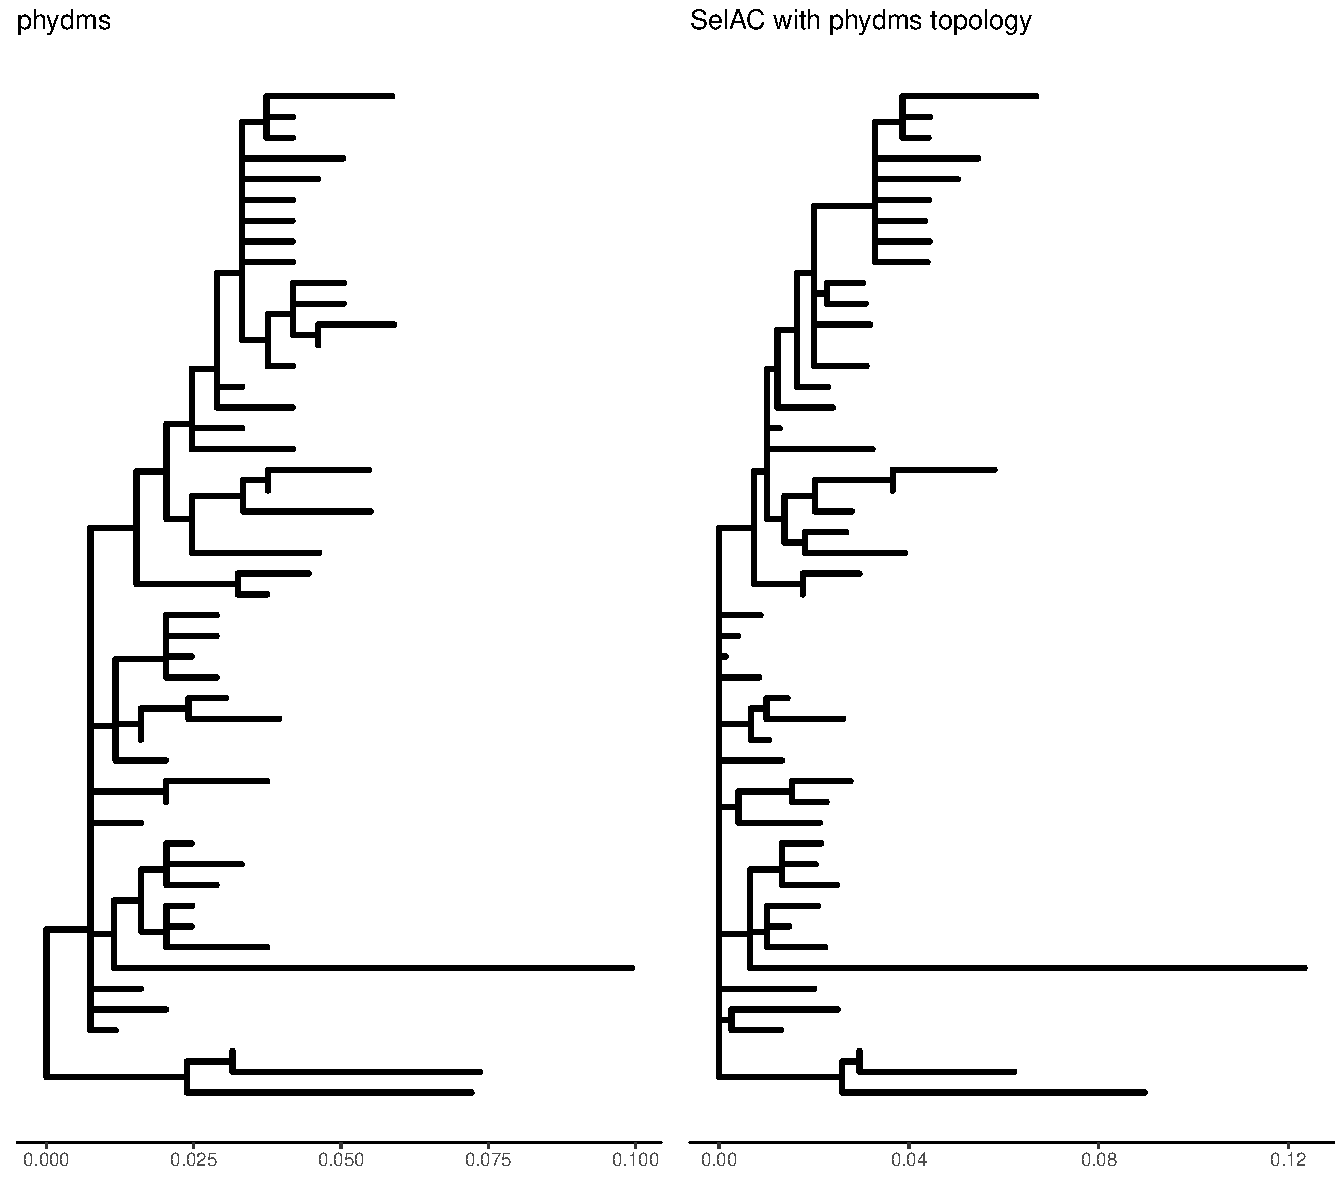
\includegraphics[width=\textwidth]{ch4/selac_top_comp.pdf}
	\caption{Phylogenies resulting from phydms, and \selac using the \phydms topology.}
	\label{fig:phylo_comp}
\end{figure}
\doublespacing
